% -*-cap2.tex-*-
% Este fichero es parte de la plantilla LaTeX para
% la realización de Proyectos Final de Carrera, protegido
% bajo los términos de la licencia GFDL.
% Para más información, la licencia completa viene incluida en el
% fichero fdl-1.3.tex

% Copyright (C) 2009 Pablo Recio Quijano 

\section{Difusión}

Este proyecto ha recibido difusión en los siguientes medios:
\begin{itemize}
    \item Forja de RedIRIS, con todo el código, documentación, tareas creadas para el proyecto, bug tracker, foros de ayuda y
            visor de archivos del sistema de control de versiones.
    \item Inclusión en la próxima versión de la distribución GNU/Linux Guadalinex v8.
    \item Finalista en la Categoría Proyectos Libres de Ocio de la Universidad de Cádiz 2009-2010~\ref{fig:cusl2}, dentro del IV
            Concurso Universitario de Software Libre.
    \item Accésit al Mejor Proyecto Libre de Innovación en la Universidad de Cádiz 2010-2011~\ref{fig:cusl1}, enmarcado en el V
            Concurso Universitario de Software Libre.
    \item Sección especial dedicada al programa dentro del portfolio personal.
    \item Página web de la Asociación de Desarrollo de Videojuegos de la UCA.
\end{itemize}

\begin{figure}[h]
  \begin{center}
    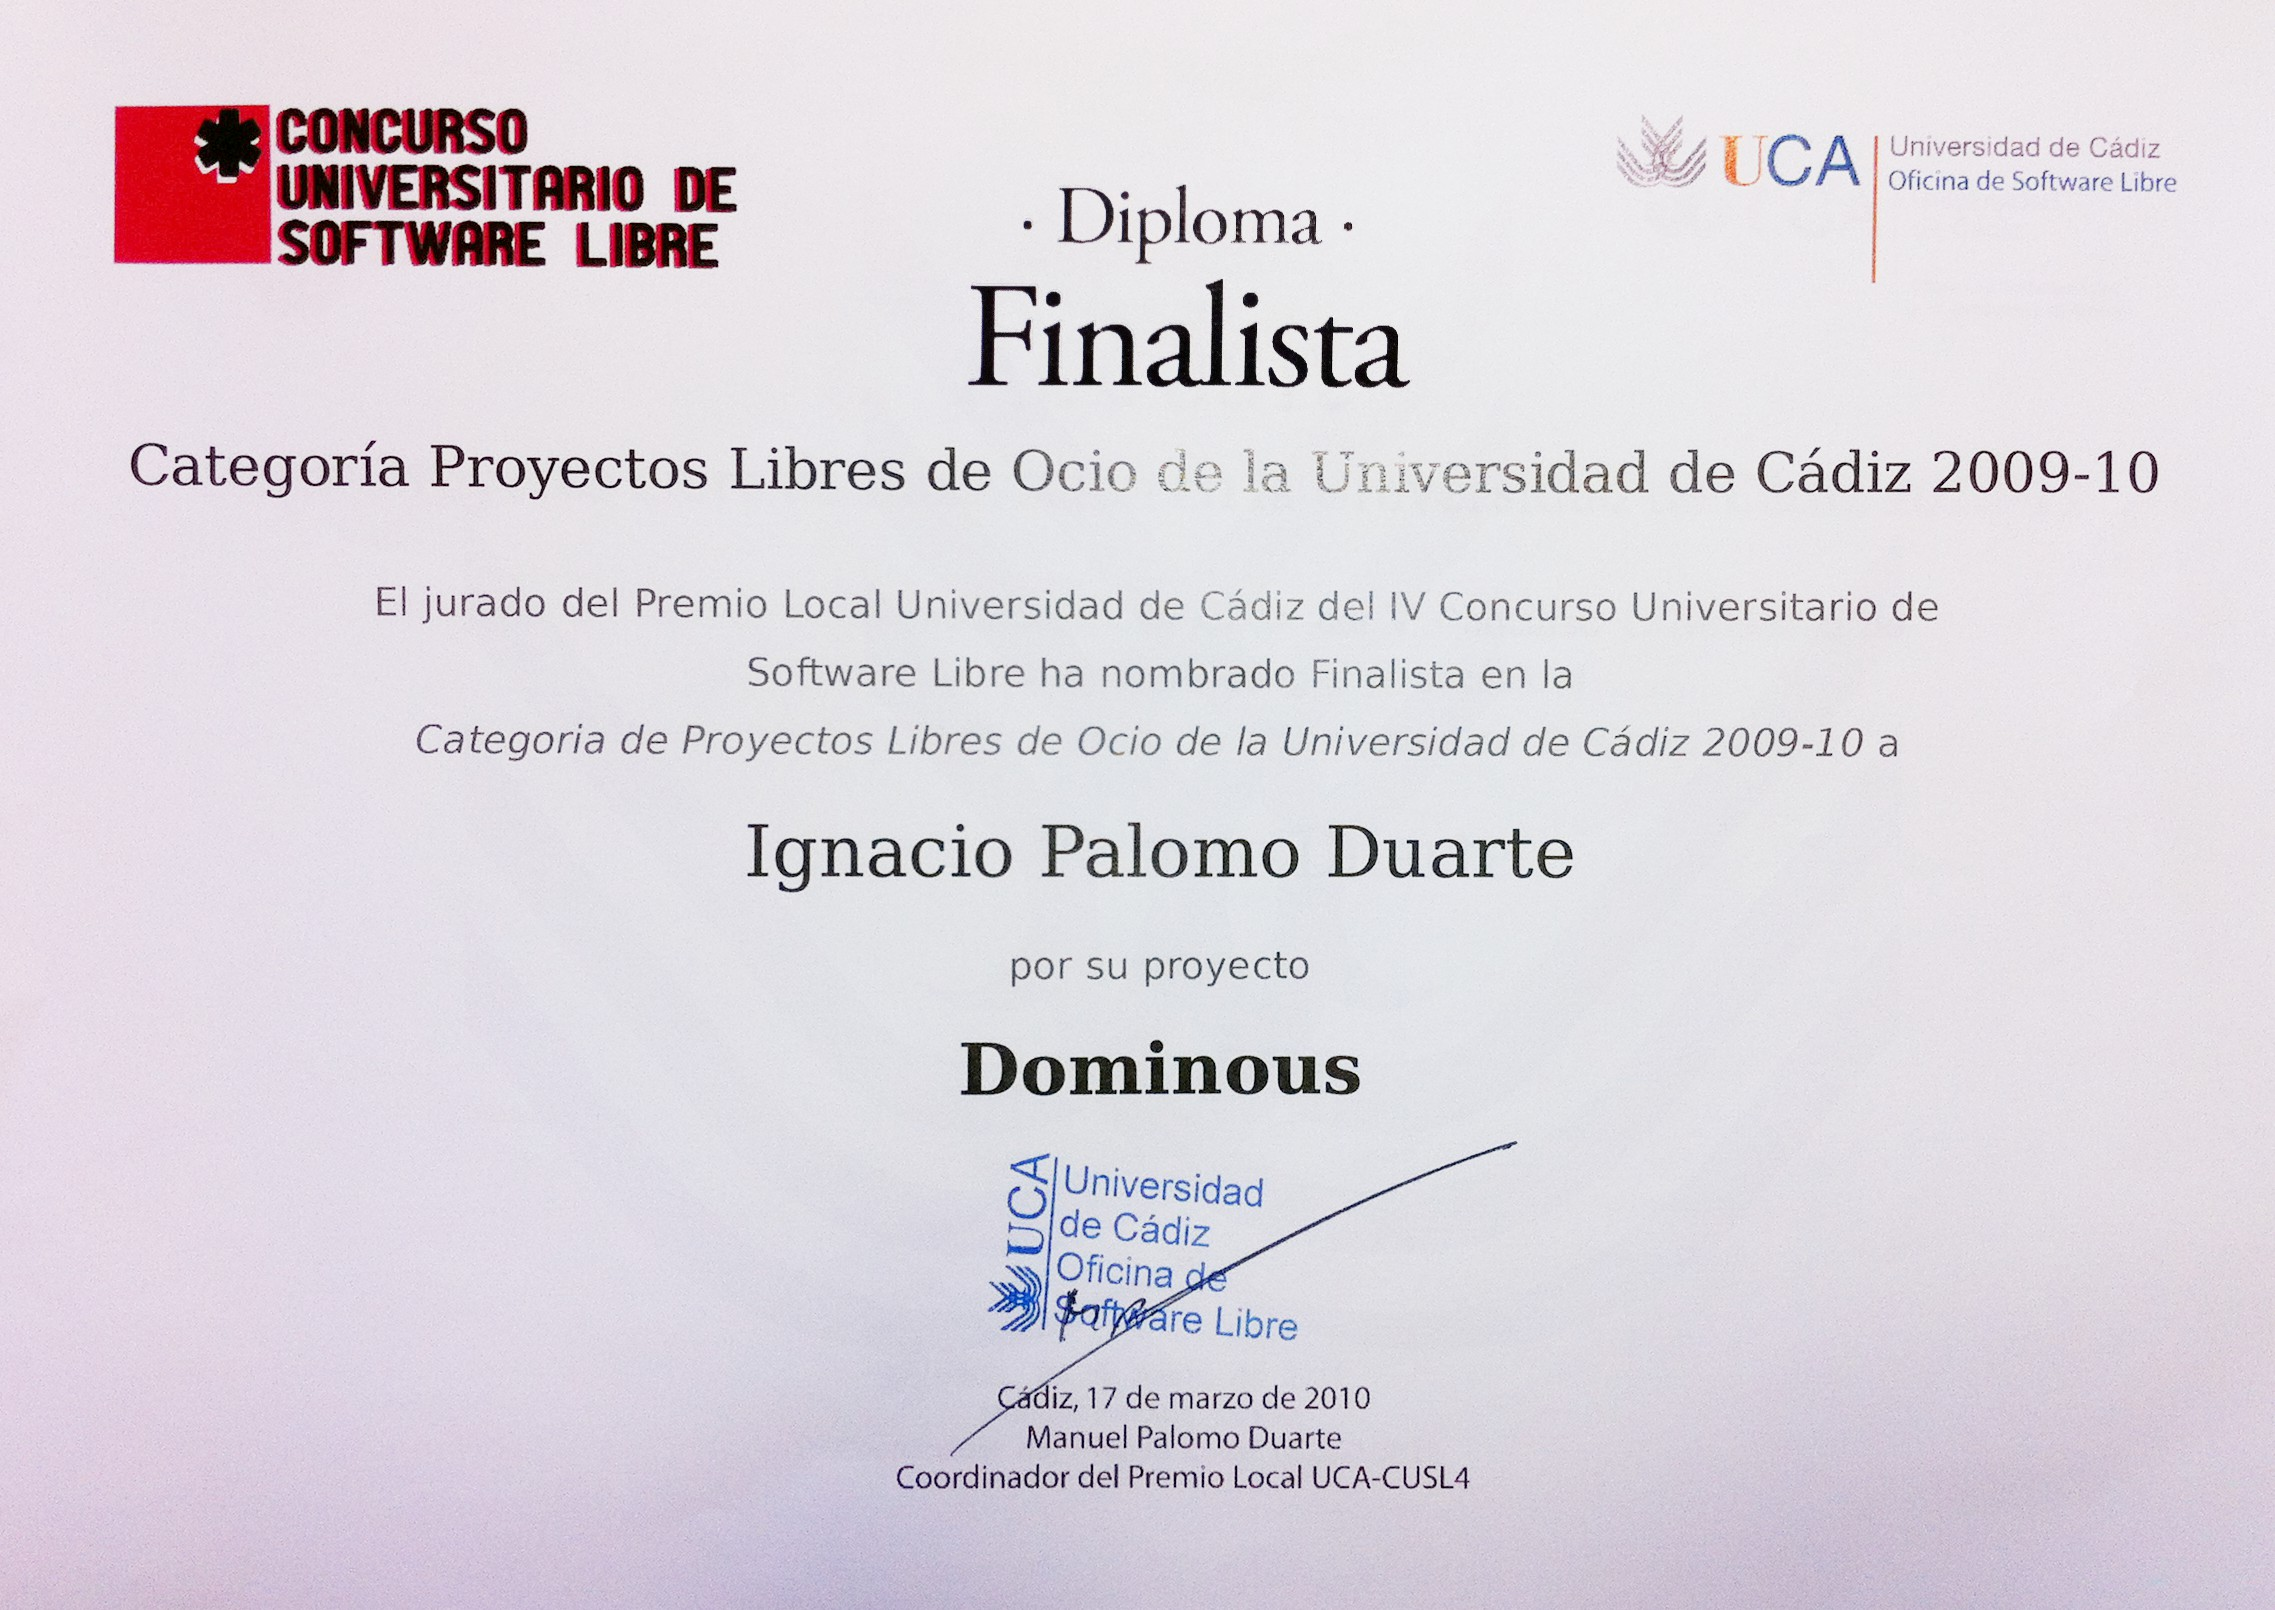
\includegraphics[scale=0.15]{CUSL2.jpg}
  \end{center}
  \caption{Finalista en la Categoría Proyectos Libres de Ocio de la Universidad de Cádiz 2009-2010}
  \label{fig:cusl2}
\end{figure}

\begin{figure}[h]
  \begin{center}
    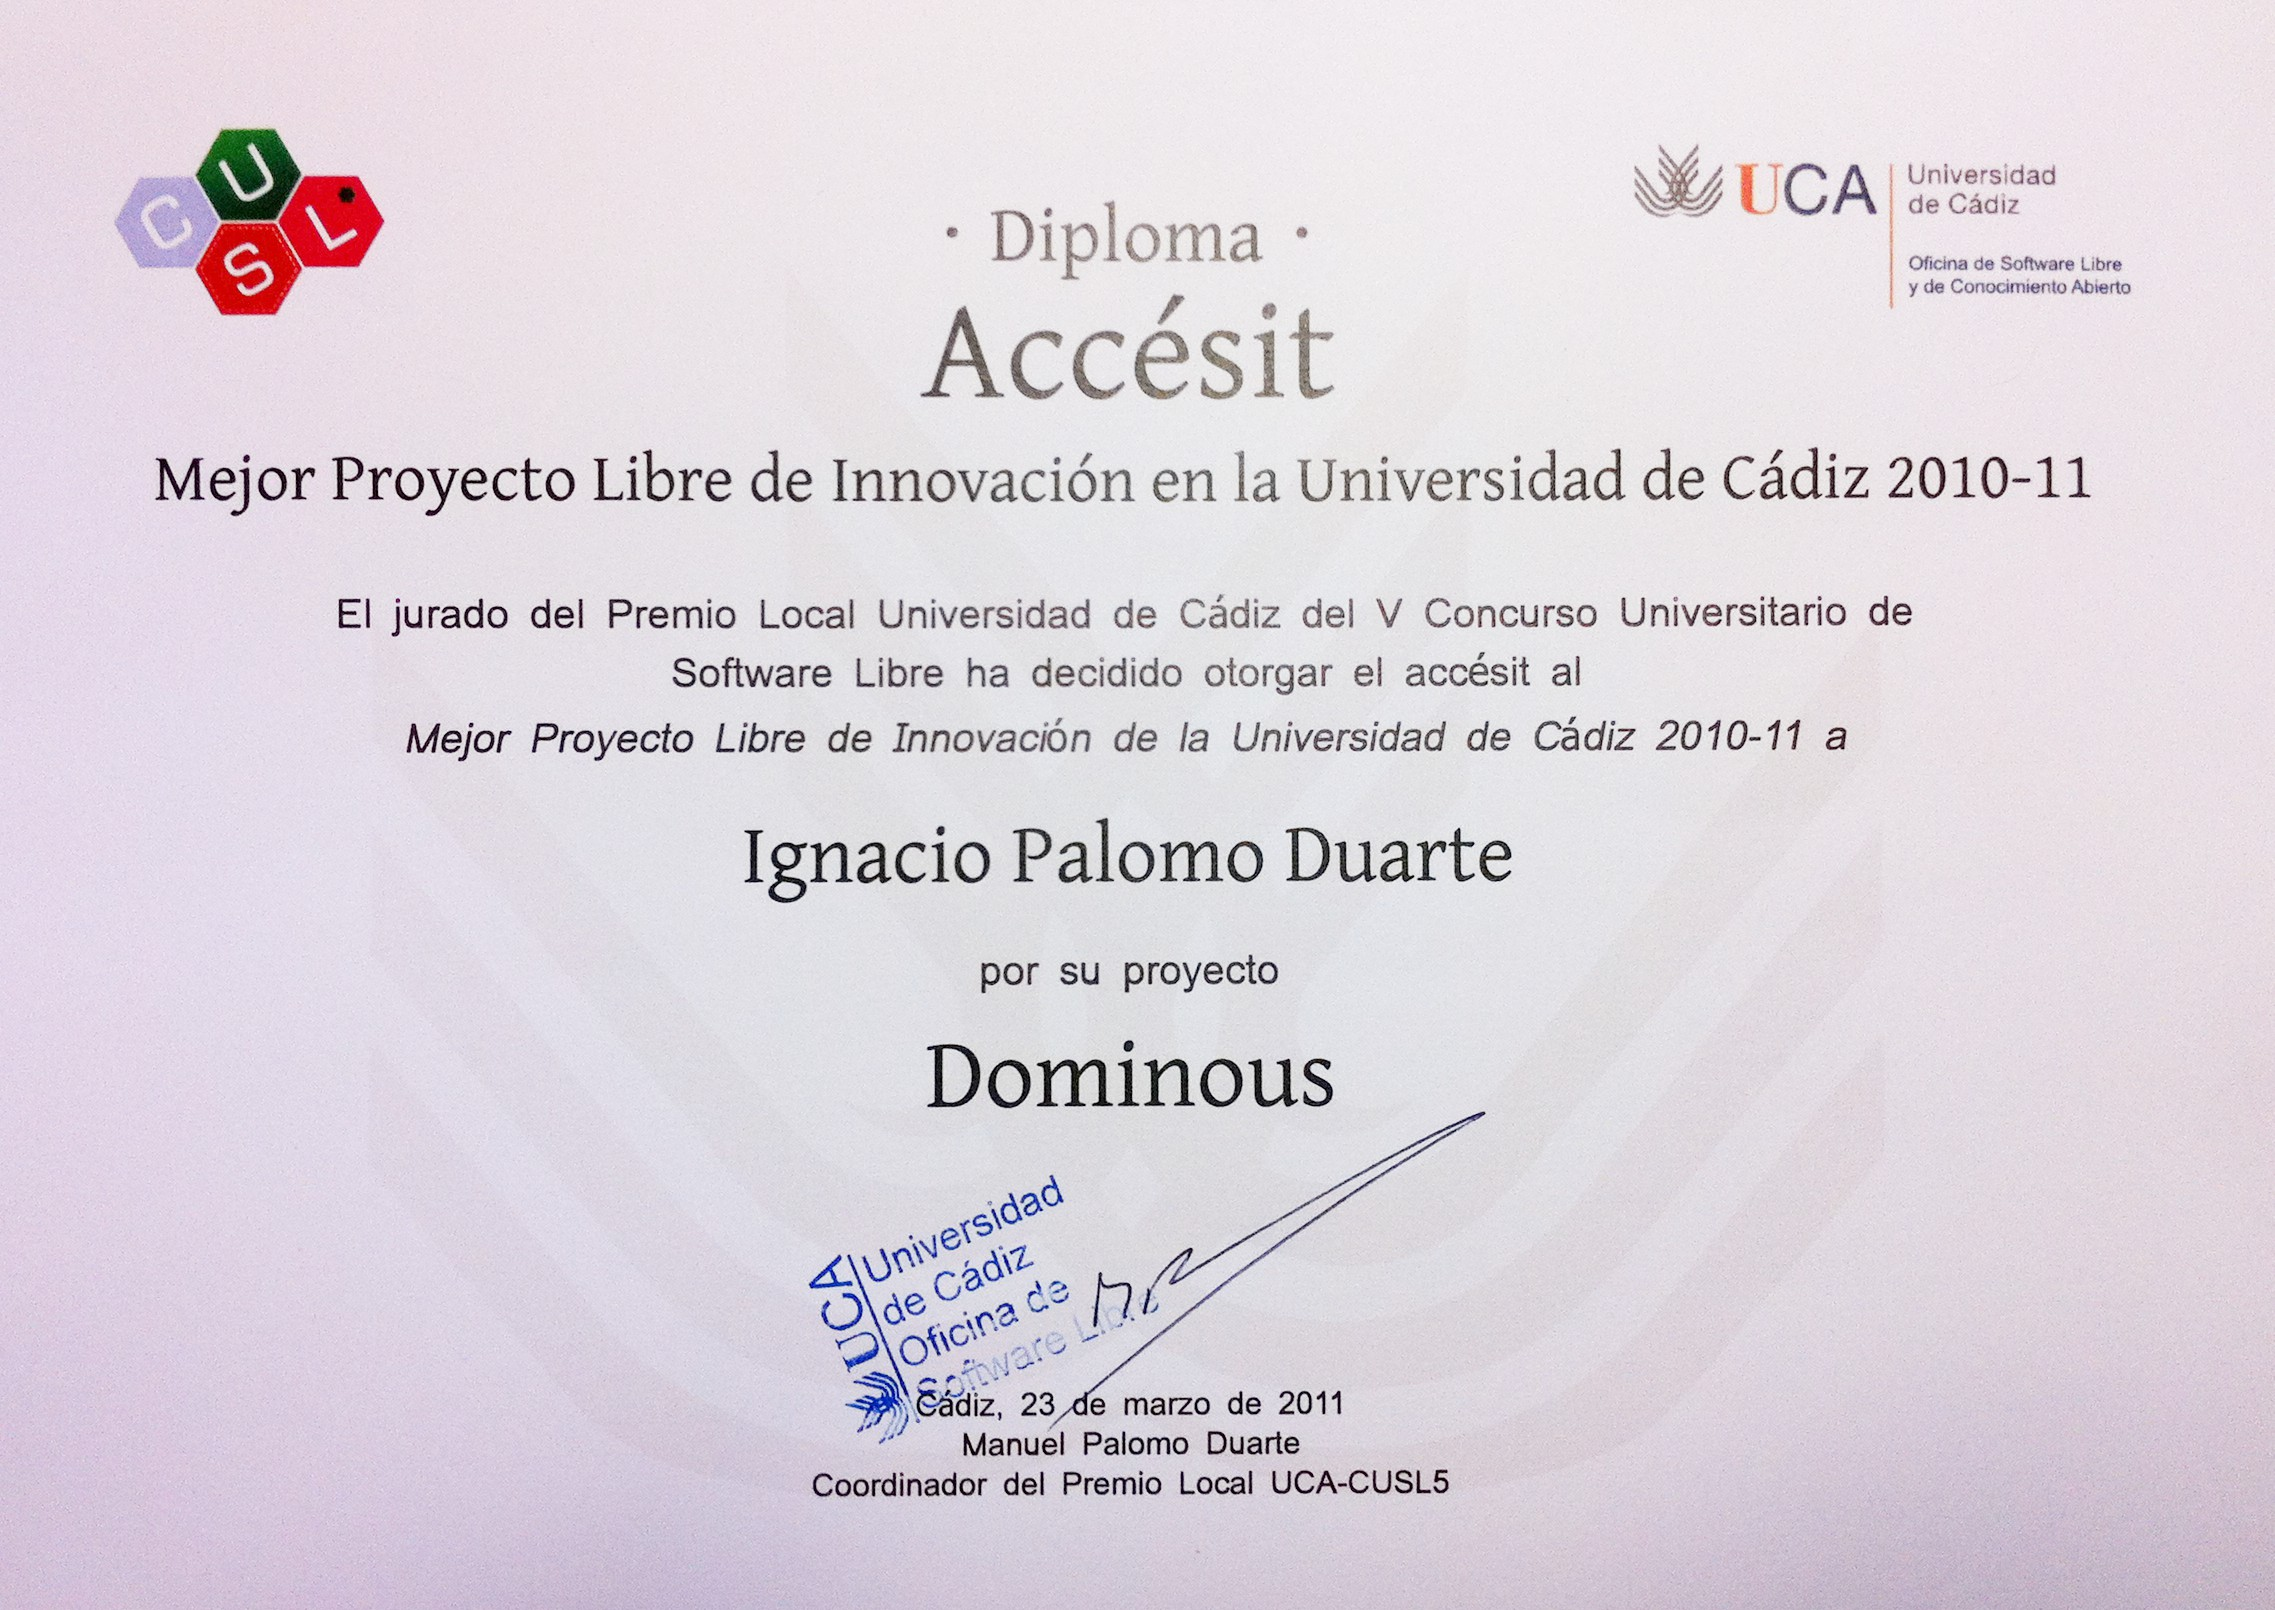
\includegraphics[scale=0.15]{CUSL1.jpg}
  \end{center}
  \caption{Accésit al Mejor Proyecto Libre de Innovación en la Universidad de Cádiz 2010-2011}
  \label{fig:cusl1}
\end{figure}


